\documentclass[12 pt]{scrartcl}
\usepackage{setspace}
\onehalfspacing
\usepackage{amsmath,amssymb,amsfonts,amsthm,mathtools}
\usepackage[english]{babel}
\usepackage[T1]{fontenc}
\usepackage[utf8x]{inputenc}
\usepackage{lmodern}
\usepackage{dsfont}
\usepackage{bbm}
\usepackage[round]{natbib}
\usepackage{color} 
\usepackage[defaultlines=2,all]{nowidow}
\usepackage{caption}
\usepackage[labelformat=simple]{subcaption}
\renewcommand\thesubfigure{(\alph{subfigure})}

\setlength\parindent{0pt}
\setlength{\parskip}{6pt plus 1pt minus 1pt}

\newcommand{\red}{\textcolor{red}}


\begin{document}



\begin{titlepage}
	\centering
	{\scshape\LARGE TU Dortmund \par}
	\vspace{1cm}
	{\scshape\Large Introductory Case Studies \par}
	\vspace{2cm}
	{\huge\bfseries Project {III}: {Regression Analysis}\par}
	\vspace{2cm}
	{\Large Lecturers:\\
		Prof.\ Dr.\ Katja Ickstadt\\
		M.\ Sc.\ Zeyu Ding\\
		M.\ Sc.\ Yassine Talleb \par}
	\vspace{1cm}
	{\Large Author: {Saptarsi Bhattacharya} \par}
	\vspace{0.5 cm}
	{\Large Group number: {5}\par}
	\vspace{0.5 cm}
	{\Large Group members: { Zahidul Islam Prince, Ikhtiar Ahmed, Saptarsi Bhattacharya}}
	\vfill
	{\large \today\par}
\end{titlepage}



\tableofcontents
\thispagestyle{empty}

\cleardoublepage

\setcounter{page}{1}

\section{Introduction}

This project focuses on the "Seoul Bike Sharing Demand Data Set" \citep{seoul} which provides valuable insights into bike rentals in Seoul, South Korea. The goal of the project is to explore the dataset, develop a predictive model, and gain a better understanding of the factors influencing bike rental counts. By examining variables such as temperature, humidity, wind speed, and seasonal variations, we aim to contribute to the improvement of bike sharing systems and resource allocation. 

To solve the problem at hand, we will follow a systematic approach. First, we will perform exploratory data analysis to comprehensively understand the dataset. This step will involve assessing the characteristics and distribution of the variables, identifying any missing values or outliers, and obtaining initial insights into their relationships. 

Next, we will conduct descriptive analysis using techniques such as scatter plots or correlation plots. This analysis will provide visualizations and statistical measures to explore the relationships between variables. By identifying potential trends or patterns, we can gain insights into the factors that impact bike rental counts. 

Succeeding the descriptive analysis, we will develop a regression model to predict the number of bike rentals. First, we will use a linear regression model using all available independent variables. Through this model, we can assess the significance of each variable and evaluate the model's performance. 

To enhance the interpretability and efficiency of the model, we will use the best subset selection technique that will guide us in identifying a subset of explanatory variables that significantly influence bike rental counts. We will consider criteria such as AIC, BIC, adjusted-R2, or Mallows' Cp values to aid in the selection process. Once the selected regression model is established, we will evaluate its performance. This evaluation will involve analyzing residual plots to assess linearity, heteroskedasticity, and normality. Additionally, we will examine the variance inflation factor (VIF) to detect and address any multicollinearity issues that may arise. The results of the regression model will be interpreted to understand the impact of the selected variables on the bike rental counts.

In conclusion, this project aims to explore the bike rental data set and develop a regression model to predict a bike rental counts. By analyzing the relationships between variables, selecting significant predictors, and interpreting the results, we seek to contribute to the improvement of bike-sharing systems in Seoul.
 


\section{Problem statement}



\subsection{Description of the data set and quality}

The "Seoul Bike Sharing Demand Data Set" \citep{seoul} provides information on bike rentals in Seoul, South Korea. The dataset was collected through an observational study over a certain period. It includes 10 independent variables and one dependent variable. The independent variables represent various factors such as the hour of the day, temperature, humidity, wind speed, visibility, solar radiation, rainfall, snowfall, seasons, and holiday. The dependent variable is the log.Rented.Bike.Count, which is the natural logarithm of the number of bike rentals in each hour. This transformation was applied to address issues with the original dependent variable, which did not follow a normal distribution and had a significant number of zeros.

While the dataset description does not provide specific details about missing values, measurement scales, and measurement accuracy, it is essential to consider these aspects when analyzing the data. Handling missing values appropriately and understanding the measurement scales of the variables is crucial for an accurate interpretation. Furthermore, measurement accuracy is an essential factor to ensure the reliability of the dataset. 

In summation, the data set is derived from an observational study and contains information about bike rentals in Seoul. The dataset's variables capture various factors that may influence bike rental demand. However, without detailed information on missing values, measurement scales, and measurement accuracy, it is necessary to exercise caution and consider these aspects when analyzing the data.


\subsection{Project objective}

The project has both content-related and statistical objectives. From a content perspective, the goal is to understand the factors influencing bike rental demand in Seoul by analyzing variables such as temperature, humidity, wind speed, visibility, solar radiation, rainfall, snowfall, seasons, and holidays. This analysis aims to optimize bike sharing systems, improve resource allocation, and enhance the user experience. 

Statistically, the project aims to develop a linear regression model to predict the bike rental counts using the available independent variables. Variable selection methods will be employed, guided by statistical criteria such as AIC, BIC, \emph{adjusted-${R^2}$}, or Mallows' \emph{Cp} values. The selected model will provide parameter estimates, statistical significance, confidence intervals, and a goodness-of-fit measure. Interpreting the regression results will offer insights into the impact of the variables on the bike rental demand, aiding in decision-making for bike-sharing system operators and policymakers.
 


\section{Statistical methods}

This section introduces statistical methods that will be used to analyze and evaluate the data set in the next section of the current report. R \citep{R} version 4.0.5 and default loaded packages are used for all data processing and visualizations.

\subsection{Classical linear regression model}

In the linear regression model, our main goal is to study the relationship and influence of a given set of explanatory variables (also known as independent variables, predictors or regressors) ${x_1, x_2,...,x_k}$ on the target variable ${y}$. In general, the linear function \emph{f$(x_1, x_2,...x_k)$} can be used to model the connection between the target and explanatory variables. The linear function is considered to have an error or noise ($\varepsilon$) in the model because the connection is not accurate, and thus we get the form below.

$y =  \emph{f$(x_1, x_2,...x_k)$} + \varepsilon$, where $\varepsilon$ is the error or the noise in the model and $f$ is the unknown function and represented as a linear combination of covariates given as, \emph{f$(x_1, x_2,...x_k)$} = ${\beta}_0 + {\beta}_1{x_{1}} + ....+ {\beta}_k{x_{k}}$.\\
Hence, the linear function can be rewritten as,\\
$y = {\beta}_0 + {\beta}_1{x_{1}} + ....+ {\beta}_k{x_{k}} + \varepsilon$, where ${\beta}_0, {\beta}_1 , ...., {\beta}_k$ are the unknown regression parameters or coefficients which need to be determined.

For $i$ = ${(1,2,...n)}$  samples, the matrix form of the regression model is given as,

\[
\textbf{y} = 
\begin{pmatrix}
{y_0}\\
\vdots\\
{y_i}
\end{pmatrix}
 \,
\boldsymbol{\varepsilon} =
\begin{pmatrix}
{\varepsilon_0}\\
\vdots\\
{\varepsilon_i}
\end{pmatrix}
\]
\[
\textbf{X} = 
\begin{pmatrix}
1 & {x_{11}} & {\cdots} & {x_{1k}}\\
\vdots & {\vdots} & {\ddots} & {\vdots}\\
1 & {x_{i1}} & {\cdots} & {x_{ik}}\\
\end{pmatrix}
 \,
\boldsymbol{\beta} =
\begin{pmatrix}
{\beta_0}\\
\vdots\\
{\beta_k}
\end{pmatrix}
\]
or, $ \textbf{y} = {\textbf{X}}{\boldsymbol{\beta}} + {\boldsymbol{\varepsilon}}$\\
where  $\textbf{y}$ is the response vector,
 $\textbf{X}$ is the design matrix,
${\boldsymbol{\beta}}$ is the unknown parameter vector and
${\boldsymbol{\varepsilon}}$ is the error vector.\citep[p.~73-75]{regression}

\subsubsection{Model assumption}

There are a few assumptions that must be addressed before using the linear regression model. A linear regression model requires that the number of observations in the data set must be equal to or larger than the number of regression coefficients, which is an important criterion.

 \begin{itemize}
\item The target and the explanatory variables must have a linear relationship. Residual vs fitted plot is used to verify this assumption.
\item No, perfect multicollinearity, which implies that any explanatory variable that is a linear modification or transformation of other explanatory variables should be avoided. This assumption could be validated using the variance inflation factor (VIF) which is discussed in subsection 3.1.4 of this report.
\item Errors are assumed to be normally distributed which can be validated using a QQ-plot. If the residuals lie on the straight reference line then it can be said that the errors follow a normal distribution Thus, $E (\varepsilon_i)$ = 0 and constant error variance $\, Var (\varepsilon_i) = {\sigma}^2$ are considered accordingly.
\item The observations or records must be independent and identically distributed {(i.i.d)}.
\end{itemize}\citep[p.~75-76]{regression}\\
All the above-mentioned assumptions with respect to the data set are verified in the next section of this report.

\subsubsection{Estimation of parameters}

The unknown regression coefficients can be estimated either by minimizing the sum of squared deviation (least squares approach) or by maximizing the likelihood estimation. 
\paragraph{Least squares method}
The least squares approach helps in estimating the unknown regression parameters by minimizing the sum of squared deviations.
$$ LS(\boldsymbol{\beta}) = \sum_{i=1}^{n}(y_{i} - \mathbf{x}_{i}^\mathbf{'}\boldsymbol{\beta})^{2} = 
\sum_{i=1}^{n}\varepsilon_{i}^{2} = \boldsymbol{\varepsilon_{i}^{'}\varepsilon}
$$

The sum of squared deviations is minimized by setting the vector of the first derivative to zero. As a result, the obtained coefficient estimator is given as:\\
${\boldsymbol{\hat{\beta}}} = {\emph{({\textbf{X}}}'\emph{\textbf{X}}\emph{)}}^{-1} \emph{{\textbf{X}}}'{\emph{{\textbf{y}}}} $.
where ${\boldsymbol{\hat{\beta}}}$ is the estimated coefficient vector. 

\paragraph{Maximum likelihood estimation}
The least square estimate does not need any specific distributional assumptions for the error term whereas the maximum likelihood estimation assumes errors to be normally distributed $\varepsilon \sim  N(0, \sigma^2I)$. Assumption of normally distributed errors, we get  the response variable vector, $y$, to be distributed normally, i.e., $y \sim N(X\beta, \sigma^2I)$ which gives the log likelihood as,

\begin{equation} \label{eq:1} l(\beta, \sigma^2)=\ - \cfrac{n}{2}log(2\pi)- \cfrac{n}{2}log(\sigma^2)-\cfrac{1}{2\sigma^2}(y-X\beta)'(y-X\beta). \end{equation}

Maximizing the above log likelihood with respect to $\beta$ is equivalent to minimizing the sum of squared deviation and gives the same result of the estimated coefficient vector as seen above. As a result, the maximum likelihood estimator of $\beta$  is equal to the least squares estimator.


From the coefficient estimator, it is also possible to compute the predicted response or target variable using the below equation.

\[
\emph{${\hat{y}}$} = {\textbf{X}}{\boldsymbol{\hat{\beta}}} = {\textbf{X}} \emph{(}{\emph{({\textbf{X}}}'\emph{\textbf{X}}\emph{)}}^{-1} \emph{{\textbf{X}}}'{\emph{{\textbf{y}}}}\emph{)}
\]
\citep[p.~105-107]{regression}
\paragraph{Residuals}

Residuals can be defined as the difference between the true {\emph{${{y_i}}$}} and the predicted value {\emph{${\hat{y_i}}$}} of the target variable. Additionally, the residuals are the estimates of errors or noise ${\varepsilon_i}$ and denoted as ${\hat{\varepsilon_i}}$.	
\[
\begin{aligned}
{\hat{\varepsilon_i}} = {\emph{${{y_i}}$}} - {\emph{${\hat{y_i}}$}} \\
or,\,\, {\boldsymbol{\hat{\varepsilon}}} = {\textbf{\emph{y}}} - {\textbf{\emph{X}}}{\boldsymbol{\hat{\beta}}}.
\end{aligned}
\]\citep[p.~77]{regression}\\
By dividing the estimated residual by the estimated standard deviation, we can obtain the standardized residual, which can then be plotted against the predicted value to see if the assumption of homoscedastic variance is broken or not. The standardized residual is computed as below:
\[
{r_i} = \frac{\hat{\varepsilon_i}}{\hat{\sigma}{\sqrt{1-h_{ii}}}}.
\]
where $h_{ii}$ are the diagonal elements of the Hat matrix H which is given as,
\[
\emph{\textbf{H}} = {\textbf{X}} \emph{(}{\emph{({\textbf{X}}}'\emph{\textbf{X}}\emph{)}}^{-1} \emph{{\textbf{X}}}'\emph{)}
\]
Hence, the predicted response variable can be rewritten as,
\[
\emph{${\hat{y}}$} = {\textbf{X}}{\boldsymbol{\hat{\beta}}} = {\textbf{X}} \emph{(}{\emph{({\textbf{X}}}'\emph{\textbf{X}}\emph{)}}^{-1} \emph{{\textbf{X}}}'{\emph{{\textbf{y}}}}\emph{)}= \emph{\textbf{Hy}}
\]
\citep[p.~124,107]{regression}

\subsubsection{Dummy encoding for categorical variables}

If the data set contains categorical variables $x_i\in {1,...,c}$ with $c$ categories, the dummy encoding is used to model the influence of these variables by introducing c-1 dummy variables in the regression model. These dummy variables can have one of the two values i.e., 0 or 1.
\[
\begin{matrix}
{x_{i1} = 
\begin{cases}
1 & \text{if } x_{i1} = 1,\\
0, & \text{otherwise,}
\end{cases}} & {\cdots} &
{x_{i,c-1} = 
\begin{cases}
1 & \text{if } x_{i,c-1} = c - 1,\\
0, & \text{otherwise}
\end{cases}}
\end{matrix}
\] 

To make the model identifiable, one of the dummy variables is omitted. For the above equation, the dummy variable for category c is removed and this category is then known as the reference category. Direct comparison with the excluded reference category is then used to interpret the effects of other dummy variables.\citep[p.~97]{regression}

\subsubsection{Collinearity analysis}

As mentioned in subsection 3.1.1, multicollinearity occurs when two or more independent or explanatory variables are correlated or linearly dependent on each other. Multicollinearity can affect the model fitting and the regression results as the model parameters become extremely sensitive to small changes in the model and as a result, it becomes hard to check explanatory variables that are statistically significant for the response variable. In order to avoid the multicollinearity issue, we use the variance influence factor (VIF) in this report. 
\paragraph{Variance influence factor}
Variance influence factor (VIF) is a technique to detect multicollinearity in regression analysis. It calculates how much multicollinearity in the model has inflated the variance of a regression coefficient. The higher the correlation between covariate $x_j$ with other covariates, the higher the coefficient of determination ${{R^2}_j}$ and hence the larger the variance $Var{\hat{\beta_j}}$. VIF is given by the below equation:
\[
VIF(\hat{\beta}j) = \frac{1}{1-{R_j}^2}\;. 
\]
where $j$=${1,2,..k}$ is the number of covariates and ${{R^2}_j}$ is the coefficient of determination of covariate ${x_j}$.

When the variance inflation factor is larger than 10, i.e., ${VIF_j}$ > 10, we state that there is a major collinearity problem.\citep[p.~157-158]{regression}

\subsubsection{Goodness of fit measure}

The extent to which the obtained model fits the data is measured by its goodness of fit. The coefficient of determination ($R^2$) is one of the goodness of fit statistics used in this project to assess the model's quality. It is computed as:	

\[
{R^2} = \frac{{\sum_{i=1}^n{{(\hat{y_i} - \bar{y})}^2}}}{\sum_{i=1}^n{{(y_i - \bar{y})}^2}} = 1 - \frac{\sum_{i=1}^n{{\hat{\varepsilon_i}}^2}}{\sum_{i=1}^n{{(y_i - \bar{y})}^2}} 
\] \citep[p.~113]{regression}

Its value varies from 0 to 1. If the $R^2$ is near to one, it means the residual sum of the square is low and the model fits the data better and $R^2$ = 1 implies that the residuals are zero with a perfect fit to the data. Additionally, we can use \emph{Adjusted} $R^2$, as an alternative of $R^2$ to avoid the false interpretation of increased $R^2$ as the number of explanatory variables increases. As a result, we include the number of explanatory variables in the computation for \emph{Adjusted} $R^2$.
\[
{\bar{R}}^2 = 1  - {\frac{n - 1}{n - k}}(1 - R^2);\,\,
\text{\,\,where\,\,k\,\,is\,\,the\,\,number\,\,of\,\,covariates.}
\] 
\citep[p.~148]{regression}

\subsection{Hypothesis testing and confidence intervals}

Using a $t$-test with a predetermined level of significance $\alpha$, the statistical significance of the regression coefficients $\hat{\beta}_j$ for $j=1,...,k$ can be evaluated under the assumption of normality of error terms, i.e., $\varepsilon_i \sim N(0,\sigma^2)$. The null hypothesis $H_0$ here is stated as none of the covariates has a significant effect on the response variable, i.e., $H_0:\hat{\beta}_j=0$, against the alternate hypothesis stated as at least one of the covariates has a significant on the response variable, i.e., $H_a:\hat{\beta}_j\neq0$ for $j=1,...,k$. The test statistics $t$ can be computed as \citep[p. 125]{regression}:
\[
t_j = \frac{\hat{\beta}_j}{se_j}\;,
\]
where $se_j = \widehat{Var(\hat{\beta}_j)^{1/2}}$ indicates the estimated standard deviation of the regression coefficients $\hat{\beta}_j$. Here, $Var(\hat{\beta}_j)$ can be obtained as \citep[p. 116]{regression}:
\[
Var(\hat{\beta}_j) = \frac{\sigma^2}{(1-R_j^2)\sum_{i=1}^{n}(x_{ij}-\bar{x}_j)^2}\;,
\]


where \(R_j^2\) here is defined as the coefficient of determination for the regression of \(x_j\) as the response and all other covariates other than \(x_j\) as predictors. \(t_j\) is a \(t\)-distributed test statistic with \(n-p\) degrees of freedom, where \(p\) is the full column rank of the design matrix \(\mathbf{X}\). The critical value of the rejection region of the null hypothesis \(H_0\) can be obtained using the \((1 - \frac{\alpha}{2})\)-quantile of the \(t\)-distribution with \(n-p\) degrees of freedom. Hence, we reject the null hypothesis if \(|t_j| > t_{n-p}(1-\frac{\alpha}{2})\). On the other hand, the p-value of the test statistic can be obtained from the \(t\)-distribution table with \(n-p\) degrees of freedom, and we reject the null hypothesis if it is less than the significance level \(\alpha\).



For linear regression coefficient estimates, a $100(1-\alpha)\%$ confidence interval specifies the interval range corresponding to $\beta_j$ for $j=0,1,...,k$ with $100(1-\alpha)\%$ percentage of probability. Under the assumption of normality of errors, the confidence intervals for a single coefficient $\beta_j$ can be constructed using the $t$-test statistic and estimated standard deviation $se_j$ as \citep[p. 136]{regression}:

\[
[\hat{\beta}_j - t_{n-p}(1-{\alpha}/{2})\cdot se_j,\; \hat{\beta}_j + t_{n-p}(1-{\alpha}/{2})\cdot se_j] \;.
\]


\subsection{Model choice criteria}

Best subset selection is a strategy that considers all possible combinations of independent variables in order to discover the subset of independent variables that best predicts the results. For $k$ different explanatory or independent variables, 2$^{k-1}$ model combinations are possible (excluding the null model). All of these models are then evaluated and the best model is selected. There exist several different techniques to select the best subset of explanatory variables such as Akaike information criteria (AIC), Bayesian information criteria (BIC), Mallow's complexity parameter etc. In this report, Akaike information criteria (AIC) is used as the model choice criteria.

\paragraph{Akaike information criteria (AIC)}

Within the scope of likelihood-based inference, the Akaike information criterion (AIC) is used for model choice. It is computed as:
\[
AIC = - 2 \cdot \emph{l}(\boldsymbol{\hat{\beta}}_k, {\hat{\sigma}}^2) + 2 (\left|{k}\,\right| + 1).
\]

Here, $\left|{k}\,\right| + 1$ is the total number of parameters and $\emph{l}(\boldsymbol{\hat{\beta}}_k, {\hat{\sigma}}^2)$ is the maximum log-likelihood (ML) value. The AIC for each regression model is calculated in order to compare them. Models with low AIC values are considered to be a better model fit.\\
In case of linear models with gaussian errors, the maximum likelihood is calculated as,\\
$- 2 \cdot \emph{l}(\boldsymbol{\hat{\beta}}_k, {\hat{\sigma}}^2) = n \,\, log({\hat{\sigma}}^2)$. \\
and the AIC is then computed as,
\[
AIC = n \,\, log({\hat{\sigma}}^2) + 2 (\left|{k}\,\right| + 1).
\]
\citep[p.~146-148]{regression}


\section{Statistical analysis}

The methods and graphs mentioned in the preceding section are applied to the dataset in this section to fit a linear model, and the results are interpreted.

\subsection{Data preparation}

Before we begin our analysis, we must first prepare our data. It starts by reading the dataset and encoding categorical variables as dummy variables. Dummy variables are created for all variables in the dataset. 

The dataset contains 2905 records and 11 variables. 

The target variable is "log.Rented.Bike.Count" and the predictor variables are "Hour," "Temperature", "Humidity", "Wind.speed", "Visibility," "Solar.Radiation", "Rainfall", "Snowfall", "Seasons" and "Holiday".

Amongst these predictor variables, two variables are categorical and the others are numerical. The categorical variables are "Seasons" with categories Spring, Summer, Autumn and Winter, and "Holiday," with categories “No Holiday” and “Holiday”.

The categorical variables are replaced by corresponding dummy variables. For "Seasons," we define three new variables "SeasonsWinter", "SeasonsSpring" and "SeasonsSummer"; each having a value '1' if the original value of "Seasons" matches with the dummy variable, '0' otherwise. For example, if the original value of Seasons is Summer, "SeasonsSummer" will have a value '1' while the other two will have a value of '0.' It is not necessary to have a dummy variable for the remaining category “Autumn” as each of these three dummy variables having a value of 0 implies that the season must be Autumn and vice versa. Here, Autumn becomes the reference category for the variable “Seasons.”

Since "Holiday" has only two possible values, only one dummy variable is required which has the value '1' if it is a Holiday and '0' otherwise.


\subsection{Descriptive analysis}


A correlation matrix is built to identify one-one correlation values between the variables.

\begin{figure}[ht]
\centering
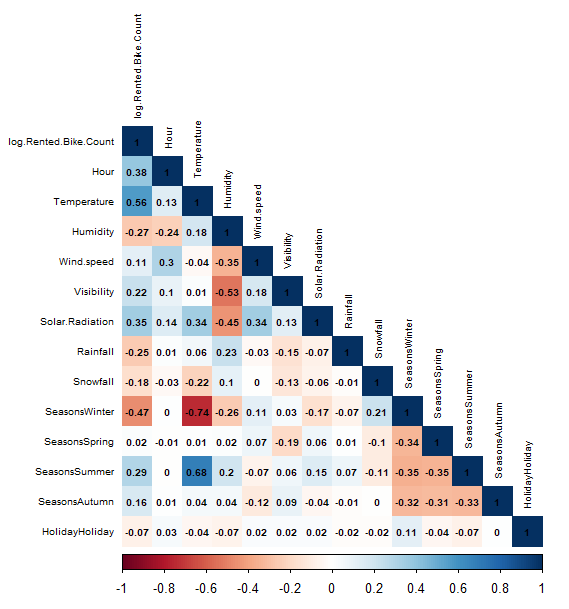
\includegraphics[width=0.8\textwidth]{Correlation plot.png}
\caption{Correlation Plot}
\label{fig: Correlation plot}
\end{figure}
\begin{itemize}
    \item Inversely correlated: "SeasonsWinter," "Humidity," "Rainfall," "Snowfall," and "holiday" have a negative correlation with log rented bike counts. This event means that bike rentals decrease during winter, high humidity, rainy days, snowy conditions, and holidays. This eventThis is understandable as these factors may discourage or inconvenience people from renting bikes.

    \item Positively correlated: "Temperature" and "Solar radiation" have a positive correlation with log rented bike counts. As temperatures rise and solar radiation increases, bike rentals tend to increase as well. This event is because warmer weather and more sunshine make for more enjoyable biking conditions.
\end{itemize}



\subsection{Response variable selection}

In the given code, the response variable is already defined as "log.Rented.Bike.Count". It is the variable that the linear regression model aims to predict. This variable is the logarithm of the count of rented bikes.

The response variable selection is crucial in regression analysis as it determines the target of the model's predictions. In this case, the logarithm of the bike count is chosen as the response variable, which can be beneficial for various reasons. Transforming the count variable to its logarithm can help address potential issues with the distribution, such as skewness or heteroscedasticity, and improve the model's performance.

By selecting the logarithm of the bike count as the response variable, the code takes into account the potential nonlinear relationship between the predictors and the actual count of rented bikes. It allows the model to capture the underlying patterns and trends more effectively, assuming that the relationship between predictors and the logged count is closer to linearity. Thus, the response variable selection in the given code, as "log.Rented.Bike.Count," demonstrates an approach to address potential challenges in modelling the count of rented bikes and to achieve a better representation of the relationship with the predictors.


\subsection{Best subset selection}

Out of all the predictor variables present, some variables may have a linear dependence on other variables (or groups of variables). We want to select only the linearly independent variables as predictors. 
The best subset selection approach fits ${2^{13} − 1}$ linear models for the 13 explanatory variables, with each possible combination of variables as a subset (excluding the empty subset) and selects the best subset of features using the AIC method. 
The best model obtained has an AIC value of 6521.45 with 9 predictors, calculated as:
log.Rented.Bike.Count \textasciitilde Hour + Temperature + Humidity + Wind.speed + Rainfall + SeasonsWinter + SeasonsSpring + SeasonsSummer + HolidayHoliday

\subsection{Estimation of the best linear model}

\begin{table}[ht]
\centering
\captionabove{Estimates of the best linear model}
\label{tab:summary}
\begin{tabular}{l|rrrr}
 & \textbf{estimate} & \textbf{std. Error} & \textbf{statistic} & \textbf{p-value}\\ 
  \hline
(Intercept) & 6.48   & 0.0740    & 87.5  & 0 \\ 
  Hour & 0.0449  & 0.00220      & 20.4  & 1.93e- 86\\ 
  Temperature & 0.0400  & 0.00239      & 16.8  & 2.88e- 60\\ 
  Humidity &  -0.0173  & 0.000771    & -22.4  & 7.79e-103\\ 
  Wind.speed &  -0.0334  & 0.0148     &  -2.26 & 2.39e-  2\\ 
  Rainfall &  -0.226  & 0.0122    &  -18.5  & 5.45e- 72\\ 
  SeasonsWinter &  -0.784  & 0.0569     & -13.8  & 7.13e- 42\\ 
  SeasonsSpring &  -0.270  & 0.0402     &  -6.70  & 2.43e- 11\\ 
  SeasonsSummer     &    -0.173  & 0.0504      & -3.44 & 5.91e-  4 \\
  Holiday &  -0.334  & 0.0635      & -5.27 & 1.49e-  7 \\ 
\end{tabular}
\end{table}

The best model with the best AIC value obtained in the above subsection is fitted and it
is interpreted using the following table. The ’estimate’ column of Table 1 shows the intercept value is 6.48, which is the value of the log.Rented.Bike.Count while all other variables remain at 0.  7 out of 9 parameter estimations are negative, inferring that with a unit increase in the parameter coefficients, a reduction in the value of log.Rented.Bike.Count by the estimated value of these coefficients can be observed (changing one variable and keeping others constant), whereas, a unit increase in positive parameter coefficients causes an increase in log.Rented.Bike.Count by the estimated value of these coefficients. For example, when the Temperature is increased by 1 unit, the log.Rented.Bike.Count increases by 0.04 units. Correspondingly, if the Humidity is increased by 1 unit, the log.Rented.Bike.Count decreases by 0.0173 units and a similar interpretation could be made for the other continuous variables. To understand the interpretation of categorical variables, let us take an example of the
variable Seasons, where Autumn is taken as the reference category and the estimate of SeasonsWinter is -0.784, which indicates that the log.Rented.Bike.Count due to Winter Season is lesser by 0.784 units to that Autumn Season, considering all other covariates remain constant. A similar interpretation could be made for other categories of categorical variables. Table 1 further shows the p-value for each parameter estimate that is obtained using
the corresponding t-statistics, which follow t-distribution with 2895 degrees of freedom. All the other coefficients have p-values less than 0.05 (given significance level) which means that the \emph(null hypothesis can be rejected) and as a result, all of these coefficients diverge considerably from 0 and have a statistically significant relationship with the response variable.



\paragraph{Confidence Interval}
The 95\% confidence intervals for the parameters are shown in Table 3 in the Appendix. Based on the test results, a confidence interval that does not include zero indicates that the coefficient is statistically significant and that the relevant explanatory variable has an effect on the response variable. It can be seen that a value of 0 does not fall within the 95\% confidence limits for all the coefficients, indicating that these variables have an effect on the response variable. 


\paragraph{Goodness of fit}
The value of ${R^2}$ or also known as the coefficient of determination is 0.5937, indicating that the model roughly explains about 59\% of the variation in the response variable. As discussed in the previous sections about the shortcomings of ${R^2}$, it is more practical to look at the adjusted ${R^2}$ value. The adjusted ${R^2}$ score is 0.5925, which is almost the same as ${R^2}$, indicating that the fitted model is quite effective. The remaining 40\% of the variation in the response variable may be due to nonlinear relationships that cannot be accurately captured by the linear regression model.


\paragraph{Linearity and Homogeneity check}
Figures 2(a) and 2(b) in the Appendix, depict the residual plot. Figure 2(a) shows a horizontal line where unevenly dispersed points form a clear cone-shaped structure, indicating a violation of the assumptions of linearity of the data and homogeneity of the residual variance.

\paragraph{Normality check}
The Q-Q plot in Figure 2(c) in the Appendix, shows that its tails deviate significantly from normality, indicating that the normality of the error distribution (one of the assumptions of classical linear regression) is violated.


\paragraph{Multicollinearity}
There exists no multicollinearity in the data set since a few explanatory factors were removed from the data set during the data preparation step because they were transformations of other explanatory variables. Consequently, each variable is distinct. The variance inflation factor (VIF) further validated the assumption of multicollinearity. The VIF values for all the variables are less than 10, indicating that there is no multicollinearity between any explanatory variables, as shown in Table 2 in the Appendix. Consequently, no explanatory variable is dropped.
\newpage

\section{Summary}

The analysis begins with data preparation, including reading the dataset and encoding categorical variables as dummy variables. The correlation matrix is computed and visualized to identify relationships between variables. A linear regression model is then fitted to predict the logarithm of the "Rented.Bike.Count" variable using various predictors. Subset selection based on the Akaike Information Criteria (AIC) is performed to determine the best combination of predictors, resulting in a model with an AIC value of 6521.45 and 9 predictors. The best model is refitted, and a summary table is generated, providing coefficients, standard errors, t-values, and p-values for each predictor.

Interpreting the best model reveals that the intercept value is 6.48, indicating the log.Rented.Bike.Count when all other variables are 0. Negative parameter estimates imply a decrease in the count with a unit increase in those predictors, while positive estimates suggest an increase. For example, a 1-unit increase in Temperature leads to a 0.04-unit increase in log.Rented.Bike.Count. Categorical variables, such as "Seasons," are interpreted using reference categories, and their estimates show the difference compared to the reference category.

The significance of the coefficients is assessed through p-values, with all coefficients, except for "SeasonsWinter," being statistically significant (p-values < 0.05). Confidence intervals are provided to indicate the precision of the parameter estimates, with intervals not including zero indicating a significant effect on the response variable.

The R-squared value, which is 0.5937, is used to measure the quality of fit and shows that the model explains 59\% of the variation in the response variable. The modified R-squared value is comparable, pointing to a fitted model that is more than successful. However, over 40\% of the variation is still unaccounted for, presumably because the linear regression model is unable to adequately account for non-linear correlations.

This analysis presents a comprehensive approach to data preparation, regression modelling, and evaluation, providing insights into the relationships between the predictor variables, and the logarithm of the rented bike count.

\newpage
\addcontentsline{toc}{section}{Bibliography}
\renewcommand\refname{Bibliography} 
\bibliographystyle{plainnat}
\bibliography{references}

\newpage
\appendix 
\addsec{Appendix}
\subsection*{A \ Additional figures}
\addcontentsline{toc}{subsection}{A \hspace*{0.15cm} Additional figures}


\begin{figure}[ht]
\begin{subfigure}{.5\textwidth}
  \centering
  % include first image
  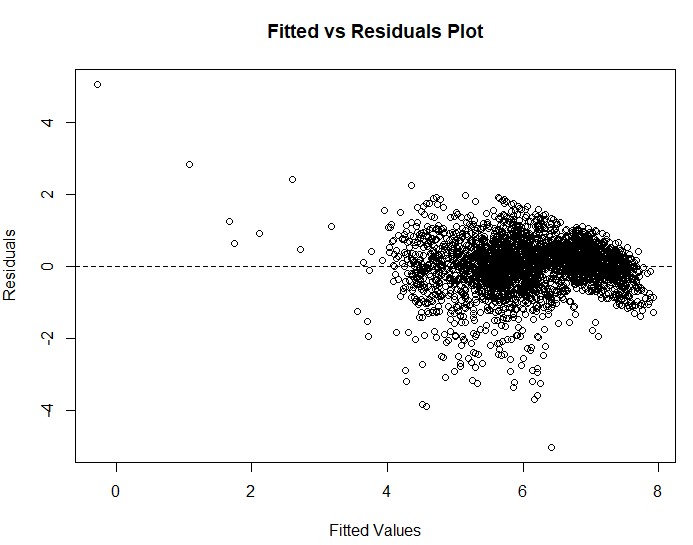
\includegraphics[height=2.6in,width=1\linewidth]{Fitted vs Residuals Plot.png}  
  \caption{Fitted vs Residuals Plot}
  \label{fig:sub-first}
\end{subfigure}
\begin{subfigure}{.5\textwidth}
  \centering
  % include first image
  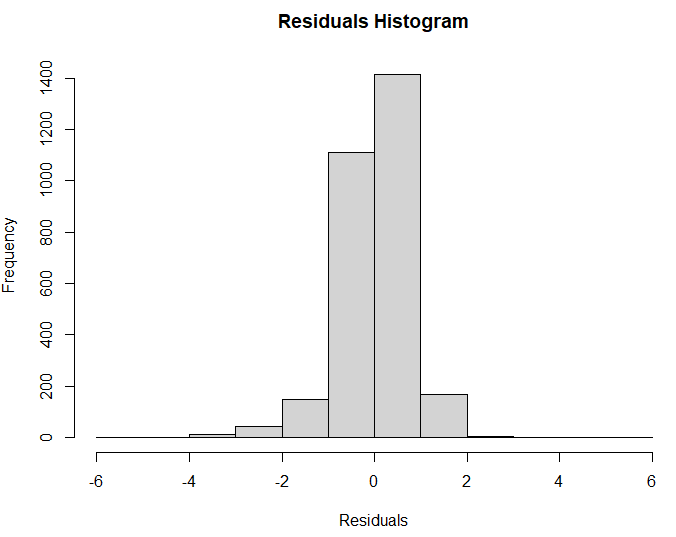
\includegraphics[height=2.6in,width=1\linewidth]{Residuals Histogram.png}  
  \caption{Residuals Histogram}
  \label{fig:sub-first}
\end{subfigure}
\begin{subfigure}{.5\textwidth}
  \centering
  % include first image
  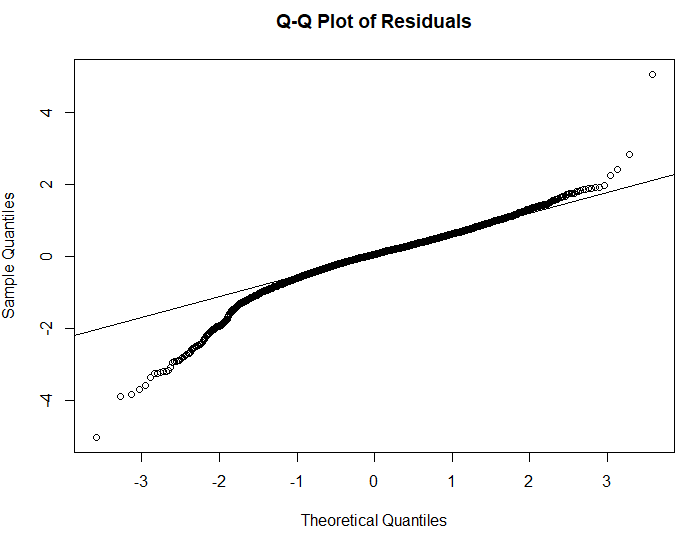
\includegraphics[height=2.6in,width=1\linewidth]{Q-Q Plot of Residuals.png}  
  \caption{Q-Q Plot of Residuals}
  \label{fig:sub-first}
\end{subfigure}
\caption{Model Diagnostic Plots}
\label{fig:fig}
\end{figure}

\newpage

\subsection*{B \ Additional tables}
\addcontentsline{toc}{subsection}{B \hspace*{0.15cm} Additional tables} 

\begin{table}[ht]
\centering
\captionabove{VIF values of the explanatory variable}
\label{description}
\begin{tabular}{c|c}
\textbf{Variable}  & \textbf{VIF} \\
\hline
Hour &  1.206633\\
Temperature  & 4.484710\\
Humidity &  1.326116\\
Wind.speed & 1.231455\\
Rainfall  & 1.062999\\
SeasonsWinter & 3.264453\\
SeasonsSpring & 1.595158\\
SeasonsSummer & 2.613082\\
HolidayHoliday & 1.029207\\
\end{tabular}
\end{table}

\begin{table}[ht]
\centering
\captionabove{Confidence Interval}
\label{description}
\begin{tabular}{c|c}
\textbf{Coefficient}  & \textbf{Confidence Interval} \\
\hline
(Intercept) & [6.33410977 , 6.624400767]\\
Hour  & [0.04056076 , 0.049193085]\\
Temperature &  [0.03532041 , 0.044677712]\\
Humidity & [-0.01879926 , -0.015776175]\\
Wind.speed  & [-0.06242092 , -0.004430582]\\
Rainfall & [-0.24998698 , -0.201968679]\\
SeasonsWinter &	[-0.89592269 , -0.672676177]\\
SeasonsSpring & [-0.34871434 , -0.190886659]\\
SeasonsSummer  & [-0.27213996 , -0.074521552]\\
HolidayHoliday  & [-0.45900735 , -0.209962611]\\
\end{tabular}
\end{table}
\end{document}